% Overall workflow (paper Fig. "Integrated modelling workflow").
% One row per model: standard input -> mathematical tool -> output, with the
% variables handed to the next model on the connecting arrows.
% Build: pdflatex workflow.tex (in this folder)
\documentclass[tikz,border=3pt]{standalone}
\usepackage{newtxtext,newtxmath}
\usepackage{amsmath,bm}
\usetikzlibrary{arrows.meta,positioning,calc,shadows}
% Shared colours for the TikZ schematics; same roles and hex values as
% Code/figures_matlab/paper_style.m (mycolor.space, base #1E5F74).
%   water (P, I, M, W-bar)  teal   | vegetation (V, r, d)  green
%   wind and sand (E, S)    brown  | highlight             orange
%   limits and caps         red dashed
\definecolor{pWater}{HTML}{1E5F74}
\definecolor{pWaterMid}{HTML}{659FB6}
\definecolor{pWaterLight}{HTML}{DCEBF1}
\definecolor{pTeal}{HTML}{00828C}
\definecolor{pVeg}{HTML}{2B633C}
\definecolor{pVegMid}{HTML}{4AC087}
\definecolor{pVegLight}{HTML}{E3F3E8}
\definecolor{pSand}{HTML}{8F7159}
\definecolor{pSandLight}{HTML}{FFEACE}
\definecolor{pAccent}{HTML}{F49431}
\definecolor{pPV}{HTML}{D47216}
\definecolor{pPVLight}{HTML}{FDF1E3}
\definecolor{pPlum}{HTML}{7A437F}
\definecolor{pPlumLight}{HTML}{F2EBF3}
\definecolor{pLimit}{HTML}{D03B3B}
\definecolor{pInk}{HTML}{1F2B33}
\definecolor{pAxis}{HTML}{344A53}
\definecolor{pGrey}{HTML}{97AFB9}
\definecolor{pGreyDark}{HTML}{647B84}
\definecolor{pGrid}{HTML}{E6EBED}

\tikzset{
  colhead/.style={font=\footnotesize\bfseries, text=pGreyDark, anchor=south},
  tab/.style={rounded corners=3pt, fill=#1, draw=none},
  inbox/.style={rounded corners=3pt, draw=#1, fill=white, line width=0.75pt,
    text=pInk, font=\footnotesize, align=left, text width=3.00cm, minimum height=1.62cm, inner sep=4pt},
  toolbox/.style={rounded corners=3pt, draw=#1, fill=#1!9, line width=0.75pt,
    text=pInk, font=\footnotesize, align=center, text width=6.25cm, minimum height=1.62cm, inner sep=4pt,
    drop shadow={opacity=0.12, shadow xshift=0.6pt, shadow yshift=-0.6pt}},
  outbox/.style={rounded corners=3pt, draw=#1, fill=#1, line width=0.75pt,
    text=white, font=\footnotesize, align=left, text width=3.40cm, minimum height=1.62cm, inner sep=4pt},
  arrow/.style={-{Stealth[length=5.5pt,width=4.5pt]}, draw=#1, line width=1.1pt},
  hand/.style={-{Stealth[length=5.5pt,width=4.5pt]}, draw=#1, line width=0.9pt, rounded corners=4pt},
  pill/.style={rounded corners=5pt, fill=white, draw=#1, line width=0.6pt, text=pInk,
    font=\scriptsize, inner xsep=5pt, inner ysep=2pt},
}
% \modelrow{y centre}{colour}{model}{task}{input}{tool name}{tool formula}{output}
\newcommand{\modelrow}[8]{%
  \fill[tab=#2] (0,#1+0.81) rectangle (1.45,#1-0.81);
  \node[text=white, font=\footnotesize\bfseries, align=center] at (0.725,#1+0.18) {#3};
  \node[text=white, font=\scriptsize, align=center] at (0.725,#1-0.30) {#4};
  \node[inbox=#2, anchor=west] (in) at (1.62,#1) {#5};
  \node[toolbox=#2] (tool) at (8.35,#1) {{\color{#2}\small\bfseries #6}\\[3pt]#7};
  \node[outbox=#2, anchor=east] (out) at (16.5,#1) {#8};
  \draw[arrow=#2] (in) -- (tool);
  \draw[arrow=#2] (tool) -- (out);
}
% \handoff{from y (row centre)}{to y}{colour}{label}
\newcommand{\handoff}[4]{%
  \draw[hand=#3] (14.6,#1-0.81) -- (14.6,{0.5*(#1+#2)}) -- (3.30,{0.5*(#1+#2)}) -- (3.30,#2+0.81);
  \node[pill=#3] at (8.95,{0.5*(#1+#2)}) {#4};
}
\begin{document}
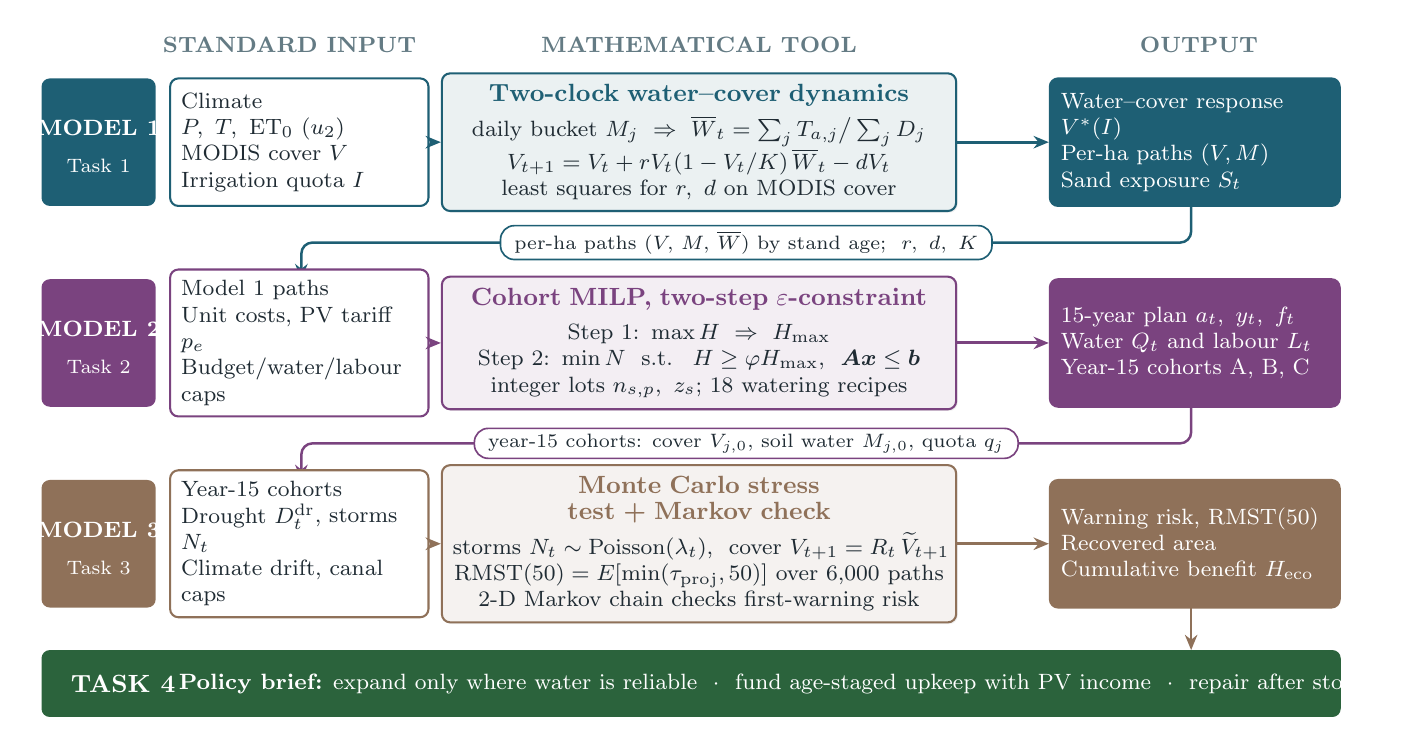
\begin{tikzpicture}
\node[colhead] at (3.15,1.02) {STANDARD INPUT};
\node[colhead] at (8.35,1.02) {MATHEMATICAL TOOL};
\node[colhead] at (14.7,1.02) {OUTPUT};

\modelrow{0}{pWater}{MODEL 1}{Task 1}
  {Climate $P,\ T,\ \mathrm{ET}_0\ (u_2)$\\MODIS cover $V$\\Irrigation quota $I$}
  {Two-clock water--cover dynamics}
  {\mbox{daily bucket $M_j\ \Rightarrow\ \overline W_t=\sum_j T_{a,j}\big/\sum_j D_j$}\\
   \mbox{$V_{t+1}=V_t+rV_t(1-V_t/K)\,\overline W_t-dV_t$}\\
   \mbox{least squares for $r,\ d$ on MODIS cover}}
  {Water--cover response $V^*(I)$\\Per-ha paths $(V,M)$\\Sand exposure $S_t$}

\handoff{0}{-2.55}{pWater}{per-ha paths $(V,\,M,\,\overline W)$ by stand age; \ $r,\ d,\ K$}

\modelrow{-2.55}{pPlum}{MODEL 2}{Task 2}
  {Model~1 paths\\Unit costs, PV tariff $p_e$\\Budget/water/labour caps}
  {Cohort MILP, two-step $\varepsilon$-constraint}
  {\mbox{Step 1: $\max H\ \Rightarrow\ H_{\max}$}\\
   \mbox{Step 2: $\min N$ \ s.t. \ $H\ge\varphi H_{\max}$, \ $\bm A\bm x\le\bm b$}\\
   \mbox{integer lots $n_{s,p},\ z_s$; 18 watering recipes}}
  {15-year plan $a_t,\ y_t,\ f_t$\\Water $Q_t$ and labour $L_t$\\Year-15 cohorts A, B, C}

\handoff{-2.55}{-5.10}{pPlum}{year-15 cohorts: cover $V_{j,0}$, soil water $M_{j,0}$, quota $q_j$}

\modelrow{-5.10}{pSand}{MODEL 3}{Task 3}
  {Year-15 cohorts\\Drought $D_t^{\mathrm{dr}}$, storms $N_t$\\Climate drift, canal caps}
  {Monte Carlo stress test + Markov check}
  {\mbox{storms $N_t\sim\mathrm{Poisson}(\lambda_t)$, \ cover $V_{t+1}=R_t\,\widetilde V_{t+1}$}\\
   \mbox{$\mathrm{RMST}(50)=\mathbb E[\min(\tau_{\mathrm{proj}},50)]$ over $6{,}000$ paths}\\
   \mbox{2-D Markov chain checks first-warning risk}}
  {Warning risk, RMST(50)\\Recovered area\\Cumulative benefit $H_{\mathrm{eco}}$}

% Task 4 bar
\draw[hand=pSand] (14.6,-5.91) -- (14.6,-6.45);
\fill[tab=pVeg] (0,-6.45) rectangle (16.5,-7.30);
\node[text=white, font=\small\bfseries, anchor=west] at (0.25,-6.875) {TASK 4};
\node[text=white, font=\footnotesize, anchor=west] at (1.62,-6.875)
  {\textbf{Policy brief:} expand only where water is reliable \ $\cdot$ \ fund age-staged upkeep with PV income \ $\cdot$ \ repair after storms};
\end{tikzpicture}
\end{document}
